\section{Model Design}

In this section, we will first introduce popular deep learning models used as baselines of our garbage dataset.

\subsection{Baselines}

We used three model architectures as our baseline of the dataset: VGGNet\cite{vgg2014}, ResNet\cite{resnet2016} and DenseNet\cite{densenet2017}. We also try the AlexNet\cite{alexnet} and SquezzeNet\cite{squeezenet2016}, but the training did not converge maybe due to the representation capacity. So we exclude these two models from our baseline list.

\subsubsection{VGGNet}

VGGNet is a Convolutional Neural Network architecture proposed by Karen Simonyan and Andrew Zisserman from the University of Oxford in 2014\cite{vgg2014}. This model mainly focuses on the effect of the convolutional neural network depth on its accuracy. This model won the 2014 ImageNet Large Scale Visual Recognition Competition, achieving an top5 accuracy of 7.1\% and top1 accuracy of 75.6\%. The architecture of VGGNet is shown in Figure \ref{fig:vgg}. VGGNet is composed of a stack of convolutional layers and 3 fully connected layers. Images directly passed through the model and the output is an 1000 dimensional vector to predict 1000 labels.
\begin{figure}[ht]
	\centering
	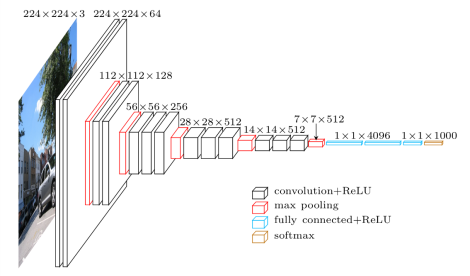
\includegraphics[scale=1.]{figs/vgg16.png}
	\caption{Architechture of VGG16\cite{vgg_arch}}
	\label{fig:vgg}
\end{figure}

The depth of VGGNet can vary by adjusting the number of convolutional layers. The model shown in Figure \ref{fig:vgg} is VGG16 composed of 13 convolutional layers and 3 fully connected layers, which add up to 16. Other popular VGG variants include VGG13 and VGG19. Batch normalization can also be added behind each convolutional layer to standardizes the inputs to a layer for each mini-batch. In the experiment, we test both classical and batch normalization version of VGG11, VGG13, VGG16 and VGG19. We find that only with batch normalization method can the VGGNet models learn the garbage dataset. Batch normalization has the effect of stabilizing the learning process and dramatically reducing the number of training epochs required to train deep networks\cite{bn_reason}.

\subsubsection{ResNet}
ResNet is proposed by Kaiming He et al.\cite{resnet2016} in 2016, which is was arguably the most groundbreaking work in the computer vision/deep learning community in the last few years. The most valuable contribution in this work is the residual learning, whose architecture is shown in Figure \ref{fig:res}. This block create a identical mapping by adding a shortcut from input to the output. The identical mapping addressed problem of vanishing/exploding gradients. In this way, a large number of convolutional layers can be stacked, leading to a powerful representation capacity.

\begin{figure}[ht]
	\begin{minipage}{0.5\linewidth}
		\centering
		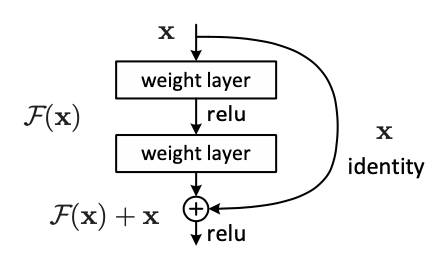
\includegraphics[width=\textwidth]{figs/residual_block.png}
		\caption{Architechture of Residual Learning\cite{resnet2016}}
		\label{fig:res}
	\end{minipage}\hfill
	\begin{minipage}{0.5\linewidth}
		\centering
		\captionof{table}{Training Condition}
		\begin{tabular}{cc}
			\toprule  % 顶部线
			Condition     & Setting   \\
			\midrule  % 中部线
			Batch Size    & 256       \\
			Epoch         & 90        \\
			Optimizer     & SGD       \\
			Learning Rate & 0.1       \\
			Momentum      & 0.9       \\
			Weight Decay  & $10^{-4}$ \\
			\bottomrule  % 底部线
		\end{tabular}
		\label{table:train_condition}
	\end{minipage}
\end{figure}


% \begin{table}[htbp]
% 	\begin{minipage}[t]{0.5\linewidth}
% 		\centering
% 		\caption{Training Condition}
% 		\begin{tabular}{cccc}
% 			\toprule  % 顶部线
% 			Condition     & Setting   \\
% 			\midrule  % 中部线
% 			Batch Size    & 256       \\
% 			Epoch         & 90        \\
% 			Optimizer     & SGD       \\
% 			Learning Rate & 0.1       \\
% 			Momentum      & 0.9       \\
% 			Weight Decay  & $10^{-4}$ \\
% 			\bottomrule  % 底部线
% 		\end{tabular}
% 	\label{table:train_condition}
% \end{minipage}
% \end{table}

By stacking different residual blocks and 1 fully connected layer, ResNet has many variants. In the experiment, we used ResNet18, ResNet50, ResNet101, ResNet152 to train and predict on our garbage dataset. The composition of these ResNet variants is show in Figure \ref{fig:res_arch}.

\begin{figure}[ht]
	\centering
	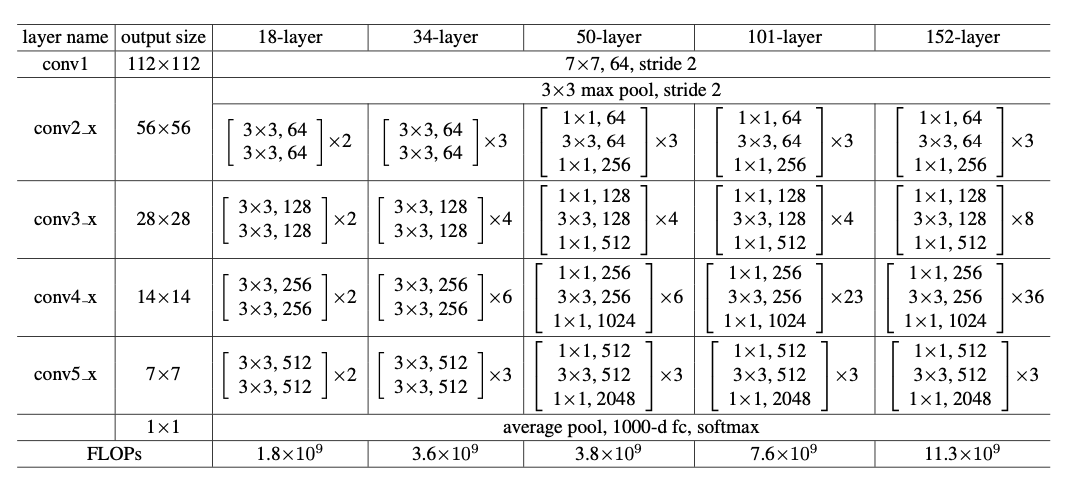
\includegraphics[width=\linewidth]{figs/resnet_arch.png}
	\caption{Architechtures of Different ResNet\cite{resnet2016}}
	\label{fig:res_arch}
\end{figure}


\subsubsection{DenseNet}
DenseNet is proposed by Gao Huang et al. \cite{densenet2017}, and won the best paper in CVPR 2017 \cite{densenet2017}. DenseNet extends the work of ResNet, building more identical shortcuts from one input to every output within the dense block. An example of a dense block with 5 convolutional layers is shown in Figure \ref{fig:dense_block}. With denser connections, DenseNet has better parameter efficiency and deeper supervision.

\begin{figure}[ht]
	\centering
	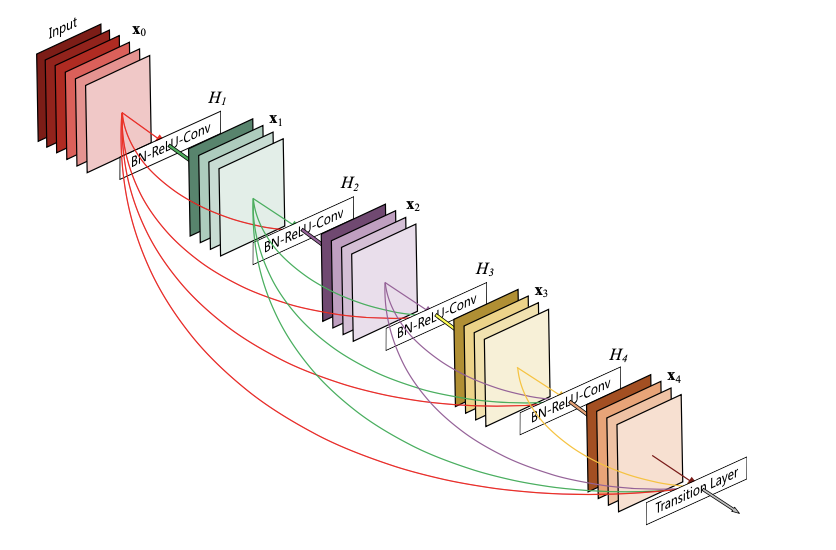
\includegraphics[width=\linewidth]{figs/dense_block.png}
	\caption{Architechtures of 5-layer Dense Block\cite{densenet2017}}
	\label{fig:dense_block}
\end{figure}

Like Resnet, the depth of DenseNet is controled by the number of stacked dense blocks. The composition of DenseNet variants is show in Figure \ref{fig:dense_arch}. In the experiment, we use DenseNet121, DenseNet161, DenseNet169 and DenseNet201 to evaluate baseline performance of DenseNet in our garbage dataset.


\begin{figure}[ht]
	\centering
	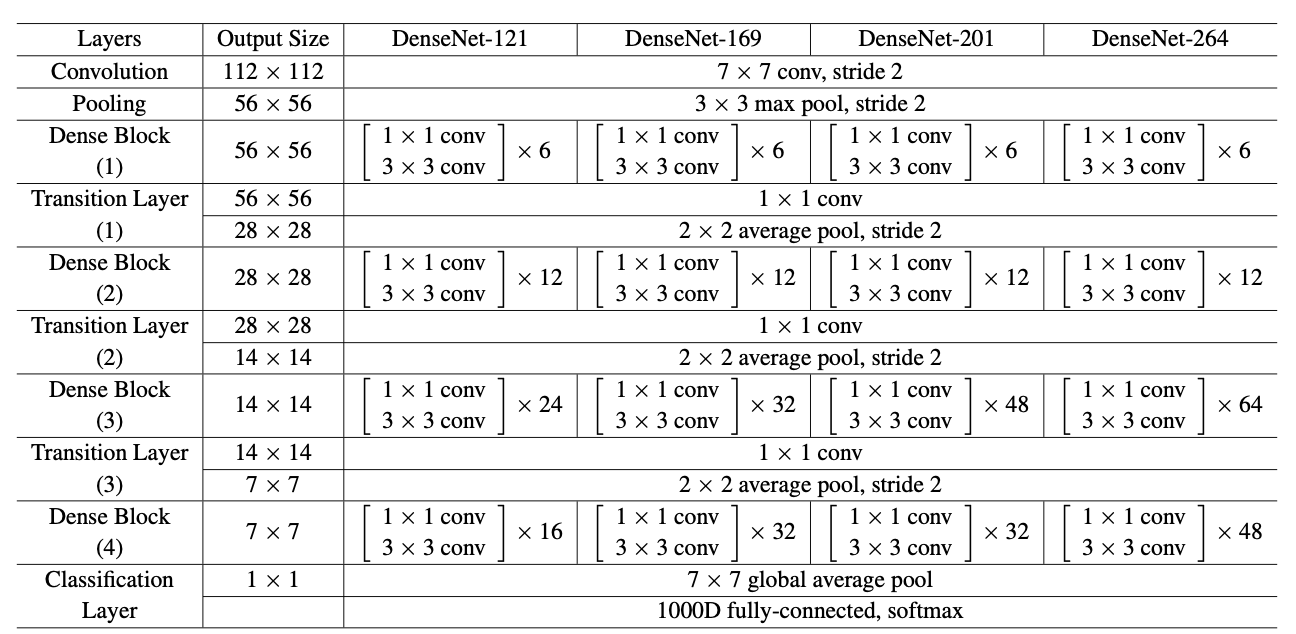
\includegraphics[width=\linewidth]{figs/dense_arch.png}
	\caption{Architechtures of DenseNet with Different Depths\cite{densenet2017}}
	\label{fig:dense_arch}
\end{figure}

\subsubsection{Experiment Setting}
We used the PyTorch version of models mentioned above, both pretrained and non-pretrained. The weights of the pretrained model have been trained on the 1000-class ImageNet dataset. We change the output channels of every model from 1000 to 42 to make the model fit to our garbage dataset. Models are trained using 10 Nvidia 2080ti GPU. Other training conditions are the same as the default settings of PyTorch official ImageNet example, which is concluded in Table \ref{table:train_condition}.
